\subsection{Template erstellen}
\begin{figure}[H]
	\centering
	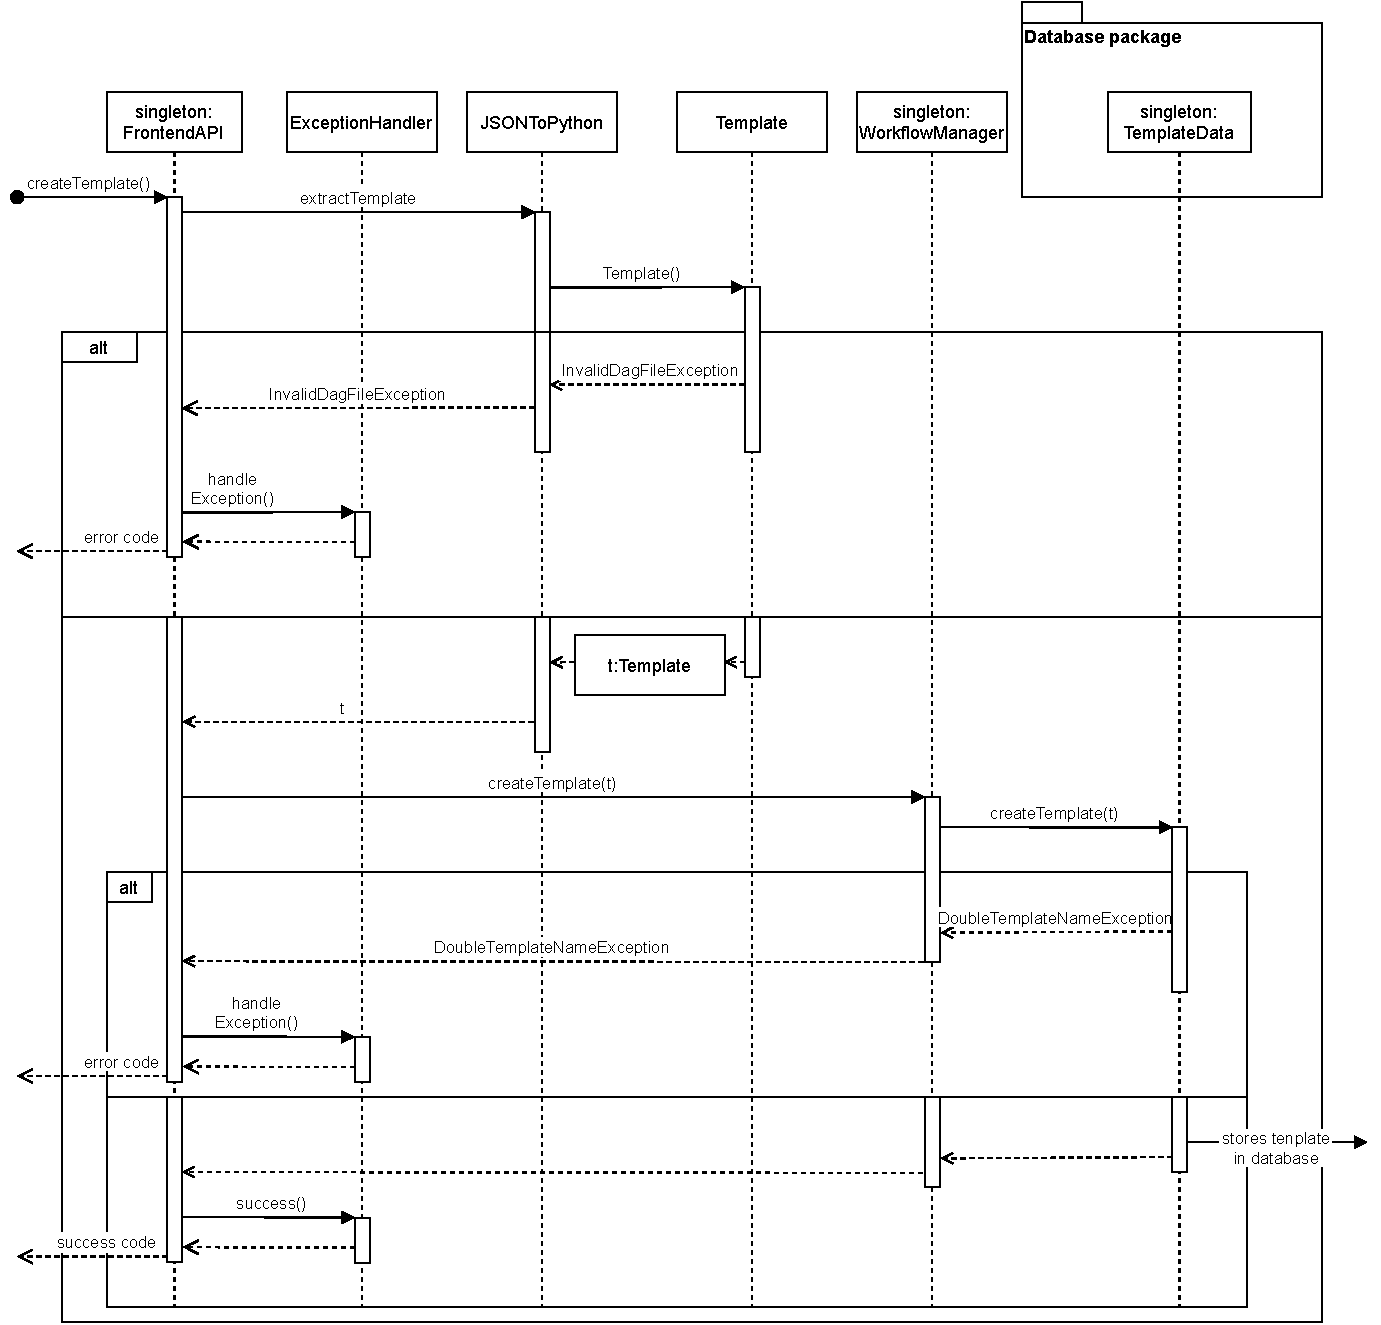
\includegraphics[width=\textwidth]{res/createTemplate.pdf} 
	\caption{Dieses Sequenzdiagramm zeigt die Erstellung eines Workflow-Templates und die dabei möglichen Fehlerfälle}
\end{figure}
Unterschieden wird zunächst der Fall, dass die dag definition file ungültig ist. Im Falle der gültigen file spaltet sich das Diagramm erneut. Zunächst wird der Fall dargestellt in dem es sich bei dem für das Template gewählten Namen um einen bereits verwendeten Bezeichner handelt. Ist der Name hingegen ein valider, identifizierender Bezeichner, wird das Template wie gewünscht erstellt.
\subsection{Workflow-Instanz erstellen}
\begin{figure}[H]
	\centering
	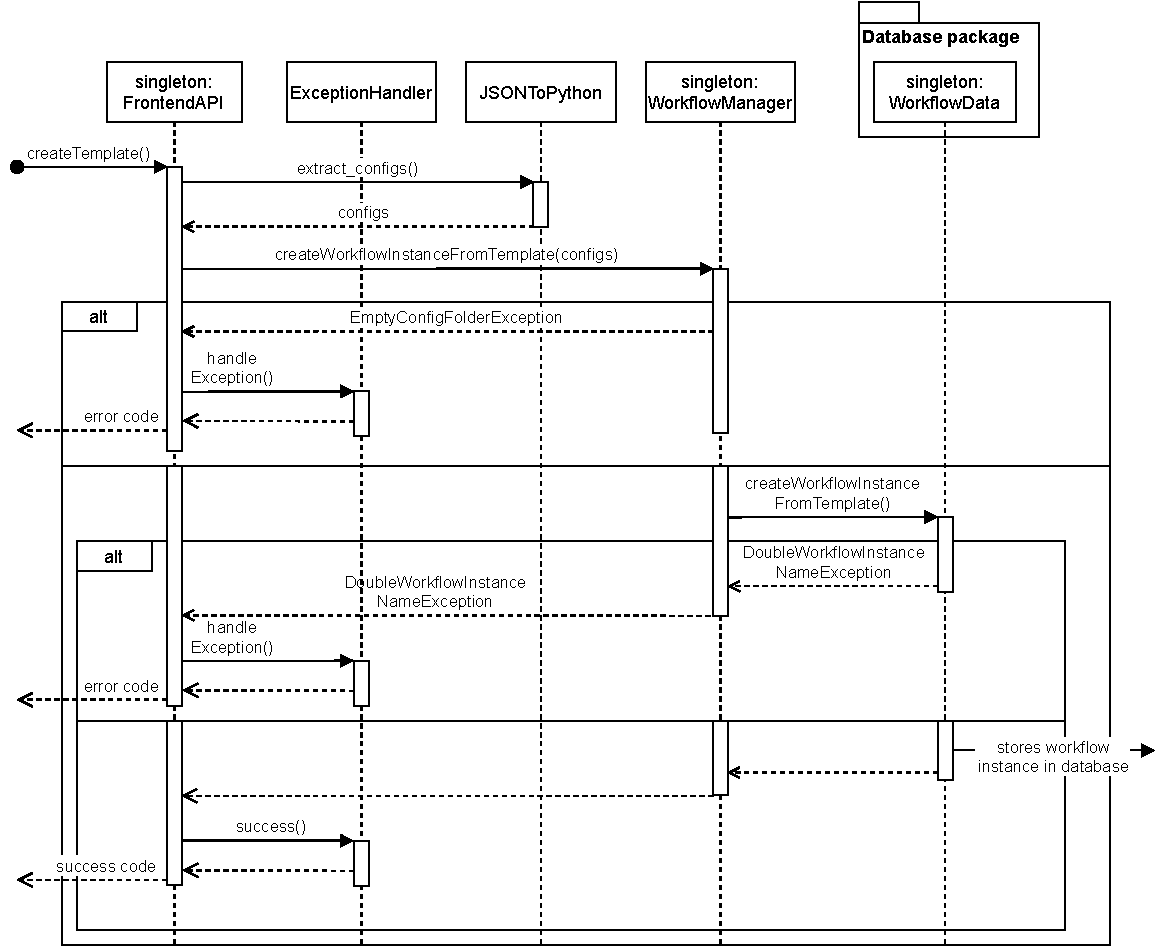
\includegraphics[width=\textwidth]{res/createWorkflowInstance.pdf} 
	\caption{Dieses Sequenzdiagramm zeigt die Erstellung einer Workflow-Instanz und die dabei möglichen Fehlerfälle}
\end{figure}
Auch in diesem Diagramm gibt es zwei Fallunterscheidungen. Zum einen kann die Erstellung an einem leeren config-Ordner, zum anderen an einem nicht eindeutigen Namen der Instanz scheitern. Treten diese Fehlerfälle nicht auf, so gelingt die Erstellung.
\subsection{Version einer Workflow-Instanz erstellen}
\begin{figure}[H]
	\centering
	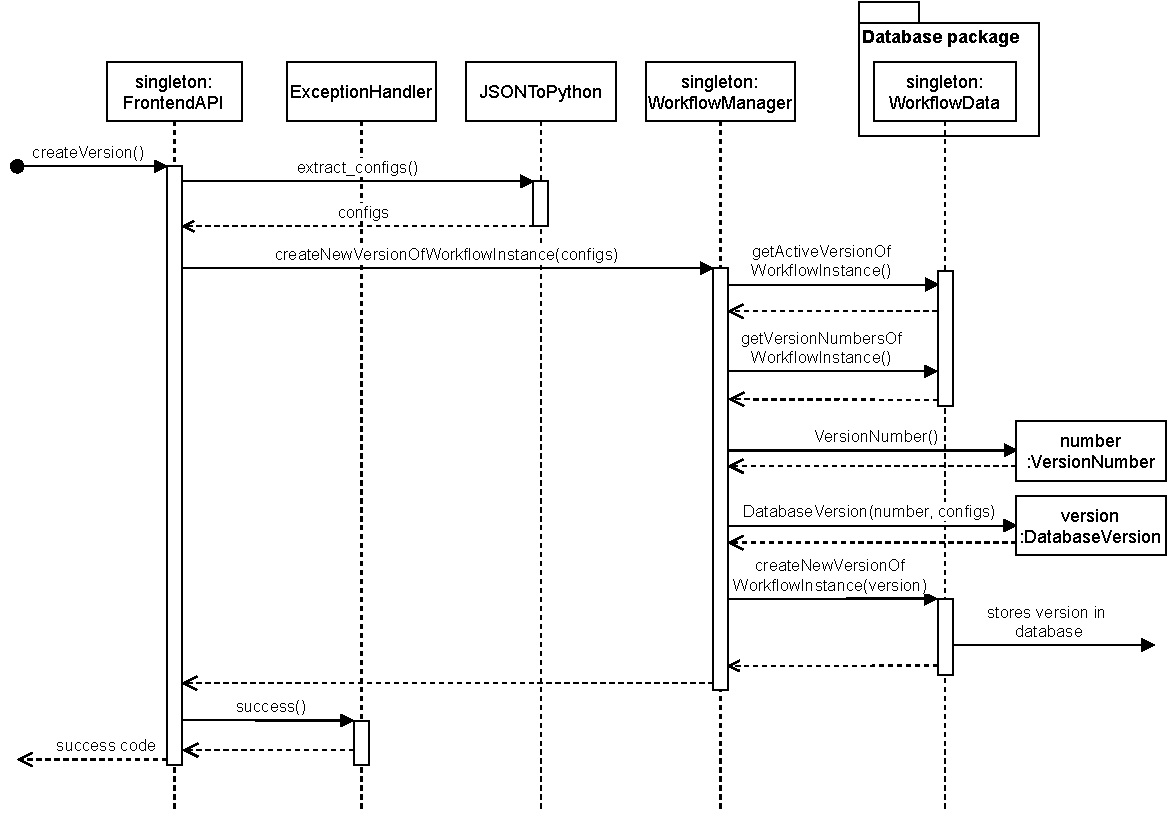
\includegraphics[width=\textwidth]{res/createVersion.pdf} 
	\caption{Dieses Sequenzdiagramm zeigt die Erstellung einer neuen Version einer Workflow-Instanz durch die Eingabe der veränderten config-flies}
\end{figure}